\subsection{Outer Measures and Caratheodory Extension}

\begin{definition} \label{def:outer-measure-generated-by-premeasure} \hlt{Outer Measure Generated by a Premeasure}\\
Let $\mu$ be a premeasure on an algebra $\mathcal{A}\subseteq\mathcal{P}(X)$. The \hlt{outer measure generated by $\mu$} is the set function $\mu^\ast:\mathcal{P}(X)\to[0,+\infty]$ defined by $\mu^\ast(B)\defeq\inf\{\sum_{j=1}^{\infty}\mu(E_j):E_j\in\mathcal{A},\ B\subseteq\bigcup_{j=1}^{\infty}E_j\}$ for $B\subseteq X$.
\end{definition}

\begin{lemma} \label{lem:generated-outer-measure-basic-properties} \hlt{Generated Outer-Measure Properties}\\
Let $\mu$ be a premeasure on an algebra $\mathcal{A}\subseteq\mathcal{P}(X)$, and let $\mu^\ast$ be as in Definition \ref{def:outer-measure-generated-by-premeasure}.
\begin{enumerate}[label=(\roman*)]
\setlength{\itemsep}{0pt}
\item $\mu^\ast(\emptyset)=0$.
\item $C\subseteq D\subseteq X\Rightarrow\mu^\ast(C)\leq\mu^\ast(D)$.
\item $(B_n)\subseteq\mathcal{P}(X)\Rightarrow\mu^\ast(\bigcup_{n=1}^{\infty}B_n)\leq\sum_{n=1}^{\infty}\mu^\ast(B_n)$.
\item $E\in\mathcal{A}\Rightarrow\mu^\ast(E)=\mu(E)$.
\end{enumerate}
\begin{proof}
\begin{enumerate}[label=(\roman*)]
\setlength{\itemsep}{0pt}
\item The cover $(\emptyset)_j$ gives $\mu^\ast(\emptyset)\leq0$, while $\mu^\ast\geq0$ by definition.
\item Every algebra cover of $D$ covers $C$; taking infima gives monotonicity.
\item If $\sum_n\mu^\ast(B_n)=+\infty$, there is nothing to prove.\\
Otherwise, for $\varepsilon>0$ choose covers $(E_{n,k})_{k\geq1}\subseteq\mathcal{A}$ of $B_n$ with $\sum_{k=1}^{\infty}\mu(E_{n,k})\leq\mu^\ast(B_n)+\varepsilon2^{-n}$.\\
Then $(E_{n,k})_{n,k}$ covers $\bigcup_nB_n$, hence $\mu^\ast(\bigcup_nB_n)\leq\sum_{n=1}^{\infty}\sum_{k=1}^{\infty}\mu(E_{n,k})\leq\sum_n\mu^\ast(B_n)+\varepsilon$; let $\varepsilon\downarrow0$.
\item For $E\in\mathcal{A}$, the cover $E,\emptyset,\emptyset,\ldots$ gives $\mu^\ast(E)\leq\mu(E)$.\\
Conversely, if $E\subseteq\bigcup_nF_n$ with $F_n\in\mathcal{A}$, set $G_n\defeq E\cap F_n\setminus\bigcup_{k<n}F_k$. Then $(G_n)$ is disjoint in $\mathcal{A}$, $\bigcup_nG_n=E$, and $\mu(E)=\sum_n\mu(G_n)\leq\sum_n\mu(F_n)$. Taking infima over covers gives $\mu(E)\leq\mu^\ast(E)$.
\end{enumerate}
\hlt{Structural Commentary}: Generated outer measures extend premeasures and are monotone and subadditive.\\
\hlt{Key Insight}: Intersect an arbitrary cover with $E$ and disjointize inside the algebra.
\end{proof}
\end{lemma}

\begin{proposition} \label{prop:single-set-envelope-vs-generated-outer-measure} \hlt{Single-Set Envelope Comparison}\\
Let $\mu$ be a premeasure on an algebra $\mathcal{A}\subseteq\mathcal{P}(X)$, and let $\mu^\ast$ be generated by $\mu$. For $B\subseteq X$, set $\mu^\sharp(B)\defeq\inf\{\mu(C):C\in\mathcal{A},\ B\subseteq C\}$. Then $\mu^\sharp|_{\mathcal{A}}=\mu$ and $\mu^\ast\leq\mu^\sharp$.
\begin{proof} If $E\in\mathcal{A}$, then $E$ is admissible, so $\mu^\sharp(E)\leq\mu(E)$. \\
Conversely, $E\subseteq C\in\mathcal{A}$ implies $\mu(E)\leq\mu(C)$; taking infima gives $\mu(E)\leq\mu^\sharp(E)$.\\
If $B\subseteq C\in\mathcal{A}$, then $C,\emptyset,\emptyset,\ldots$ covers $B$, so $\mu^\ast(B)\leq\mu(C)$. Taking infima over $C$ gives $\mu^\ast(B)\leq\mu^\sharp(B)$.\\
\hlt{Structural Commentary}: One-set envelopes dominate generated outer measures.\\
\hlt{Key Insight}: A single algebra superset is a countable algebra cover.
\end{proof}
\end{proposition}

\begin{figure}[H]
  \centering
  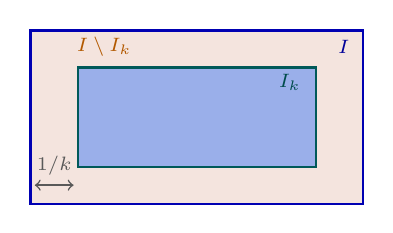
\begin{tikzpicture}[
  scale=0.88,
  every node/.style={font=\scriptsize},
  outerfill/.style={fill=blue!65, fill opacity=0.08, draw=none},
  outerline/.style={draw=blue!70!black, line width=0.85pt},
  inner/.style={fill=teal!45!blue, fill opacity=0.20, draw=teal!70!black, line width=0.85pt},
  collar/.style={fill=orange!65, fill opacity=0.20, draw=none},
  measure/.style={<->, gray!70!black, line width=0.55pt}
]
  \path[outerfill] (-2.40,-1.25) rectangle (2.40,1.25);
  \path[collar, even odd rule]
    (-2.40,-1.25) rectangle (2.40,1.25)
    (-1.72,-0.72) rectangle (1.72,0.72);
  \path[inner] (-1.72,-0.72) rectangle (1.72,0.72);

  \draw[outerline] (-2.40,-1.25) rectangle (2.40,1.25);
  \draw[inner] (-1.72,-0.72) rectangle (1.72,0.72);

  \draw[measure] (-2.34,-0.98) -- (-1.78,-0.98)
    node[midway, above] {$1/k$};

  \node[blue!60!black] at (2.12,1.02) {$I$};
  \node[teal!60!black] at (1.34,0.50) {$I_k$};
  \node[orange!70!black] at (-1.34,1.02) {$I\setminus I_k$};
\end{tikzpicture}

  \caption{Inner cells $I_k$ exhaust $I$; the collar $I\setminus I_k$ has vanishing volume.}
  \label{fig:open-cell-inner-shrink}
\end{figure}

\begin{example} \label{ex:single-set-envelope-not-outer-measure} \hlt{Single-Set Envelopes Need Not Be Outer Measures}\\
Let $X$ be uncountable, let $\mathcal{A}$ be the finite--cofinite algebra on $X$, and set $\mu(E)\defeq0$ for finite $E$, $\mu(E)\defeq+\infty$ for cofinite $E$. Then $\mu$ is a premeasure, $\mu^\ast(B)=0$ iff $B$ is countable, and $\mu^\sharp(B)=0$ iff $B$ is finite.\\
For any countably infinite $S\subseteq X$, $\mu^\sharp(S)=+\infty$ while $S=\bigcup_{x\in S}\{x\}$ and $\sum_{x\in S}\mu^\sharp(\{x\})=0$, QED.\\
\hlt{Structural Commentary}: Countable covers can be strictly smaller than one-set covers.\\
\hlt{Key Insight}: Outer measure is built from countable covers precisely to recover countable subadditivity.
\end{example}

\begin{theorem} \label{thm:generated-caratheodory-extension} \hlt{Generated Caratheodory Extension}\\
Let $\mu$ be a premeasure on an algebra $\mathcal{A}\subseteq\mathcal{P}(X)$, let $\mu^\ast$ be generated by $\mu$,\\
and set $\mathcal{C}_\mu\defeq\{E\subseteq X:\forall B\subseteq X, \mu^\ast(B)=\mu^\ast(B\cap E)+\mu^\ast(B\setminus E)\}$.\\
Then $\mathcal{A}\subseteq\mathcal{C}_\mu$, $\mathcal{C}_\mu$ is a complete $\sigma$-algebra, and $\mu^\ast|_{\mathcal{C}_\mu}$ is a measure extending $\mu$.
\begin{proof}
Lemma \ref{lem:generated-outer-measure-basic-properties} makes $\mu^\ast$ an outer measure; Theorem \ref{thm:caratheodory-measurable-sets-sigma-algebra} makes $\mathcal{C}_\mu$ a $\sigma$-algebra, makes $\mu^\ast|_{\mathcal{C}_\mu}$ a measure, and gives completeness through zero sets. Let $E\in\mathcal{A}$ and $B\subseteq X$.\\
Subadditivity gives $\mu^\ast(B)\leq\mu^\ast(B\cap E)+\mu^\ast(B\setminus E)$.\\
Conversely, if $B\subseteq\bigcup_nF_n$ with $F_n\in\mathcal{A}$, then $F_n\cap E,F_n\setminus E\in\mathcal{A}$ and $\mu(F_n)=\mu(F_n\cap E)+\mu(F_n\setminus E)$, hence $\mu^\ast(B\cap E)+\mu^\ast(B\setminus E)\leq\sum_n\mu(F_n)$. Infimizing over covers gives the reverse inequality, so $E\in\mathcal{C}_\mu$.\\
Thus $\mathcal{A}\subseteq\mathcal{C}_\mu$, and Lemma \ref{lem:generated-outer-measure-basic-properties} gives $\mu^\ast|_{\mathcal{A}}=\mu$.\\
\hlt{Structural Commentary}: Caratheodory equality is the additivity domain.\\
\hlt{Key Insight}: Every algebra set is a clean splitter for the outer measure it generated.
\end{proof}
\end{theorem}

\begin{proposition} \label{prop:caratheodory-splitters-finite-subadditive-size} \hlt{Caratheodory Splitters for Finitely Subadditive Size}\\
Let $\alpha:\mathcal{P}(X)\to[0,+\infty)$ satisfy $0\leq\alpha(E)\leq\alpha(E\cup F)\leq\alpha(E)+\alpha(F)$ for all $E,F\subseteq X$,\\
and set $\mathcal{S}\defeq\{E\subseteq X:(\forall A\subseteq X)\alpha(A)=\alpha(A\cap E)+\alpha(A\setminus E)\}$.
\begin{enumerate}[label=(\roman*)]
\setlength{\itemsep}{0pt}
\item If $\mathcal{S}\neq\emptyset$, then $\mathcal{S}$ is an algebra on $X$.
\item If $E,F\in\mathcal{S}$ and $E\cap F=\emptyset$, then $\alpha(E\cup F)=\alpha(E)+\alpha(F)$.
\item Nonemptiness is necessary: $\alpha\equiv1$ gives $\mathcal{S}=\emptyset$.
\end{enumerate}
\begin{proof}
\begin{enumerate}[label=(\roman*)]
\setlength{\itemsep}{0pt}
\item Choose $E_0\in\mathcal{S}$. Taking $A=\emptyset$ gives $\alpha(\emptyset)=0$, hence $\emptyset,X\in\mathcal{S}$. If $E\in\mathcal{S}$, the defining equality is symmetric in $E$ and $X\setminus E$, so $X\setminus E\in\mathcal{S}$. If $E,F\in\mathcal{S}$ and $A\subseteq X$, applying $F$ to $A$ and $A\setminus(E\cap F)$ and applying $E$ to $A\cap F$ gives $\alpha(A)=\alpha(A\cap E\cap F)+\alpha(A\setminus(E\cap F))$; hence $E\cap F\in\mathcal{S}$. Complements give finite unions.
\item Apply the defining equality for $E$ to $A=E\cup F$: $\alpha(E\cup F)=\alpha(E)+\alpha(F)$.
\item If $\alpha\equiv1$ and $E\in\mathcal{S}$, taking $A=\emptyset$ gives $1=1+1$, impossible.
\end{enumerate}
\hlt{Structural Commentary}: The Caratheodory splitting equation is already Boolean at the finite level.\\
\hlt{Key Insight}: Nonempty splitters force $\alpha(\emptyset)=0$; without that, the clean-splitting class may vanish.
\end{proof}
\end{proposition}

\begin{theorem} \label{thm:sigma-finite-generated-extension-uniqueness} \hlt{$\sigma$-Finite Generated Extensions Are Unique}\\
Let $\mu$ be a premeasure on an algebra $\mathcal{A}\subseteq\mathcal{P}(X)$, let $\mu^\ast$ be generated by $\mu$, and let $\mathcal{C}_\mu$ be as in Theorem \ref{thm:generated-caratheodory-extension}.\\
If $X=\bigcup_nF_n$ with $F_n\in\mathcal{A}$ and $\mu(F_n)<+\infty$, then $\mu^\ast|_{\mathcal{C}_\mu}$ is the unique measure $\nu$ on $\mathcal{C}_\mu$ satisfying $\nu|_{\mathcal{A}}=\mu$.
\begin{proof}
Existence is Theorem \ref{thm:generated-caratheodory-extension}. For uniqueness, let $\nu$ be a measure on $\mathcal{C}_\mu$ with $\nu|_{\mathcal{A}}=\mu$.\\
If $\mu(X)<+\infty$, then for $E\in\mathcal{C}_\mu$ and every algebra cover $E\subseteq\bigcup_nA_n$, $\nu(E)\leq\sum_n\mu(A_n)$, hence $\nu(E)\leq\mu^\ast(E)$.\\
Applying this to $X\setminus E$ and using $\nu(E)+\nu(X\setminus E)=\nu(X)=\mu(X)=\mu^\ast(E)+\mu^\ast(X\setminus E)$ forces $\nu(E)=\mu^\ast(E)$.\\
In general, set $H_n\defeq\bigcup_{j=1}^{n}F_j$. The finite case on $\mathcal{A}|_{H_n}\defeq\{A\cap H_n:A\in\mathcal{A}\}$ gives $\nu(E\cap H_n)=\mu^\ast(E\cap H_n)$; since $E\cap H_n\uparrow E$, continuity from below gives $\nu(E)=\mu^\ast(E)$.\\
\hlt{Structural Commentary}: Uniqueness reduces to finite-mass exhaustions.\\
\hlt{Key Insight}: Existence is Caratheodory; uniqueness needs a finite-mass exhaustion.
\end{proof}
\end{theorem}

\begin{corollary} \label{cor:sigma-finite-premeasure-unique-on-generated-sigma-algebra} \hlt{Uniqueness on the Generated $\sigma$-Algebra}\\
Let $\mu$ be a premeasure on an algebra $\mathcal{A}\subseteq\mathcal{P}(X)$. If $X=\bigcup_nF_n$ with $F_n\in\mathcal{A}$ and $\mu(F_n)<+\infty$, then any measures $\nu_1,\nu_2$ on $\sigma(\mathcal{A})$ with $\nu_1|_{\mathcal{A}}=\nu_2|_{\mathcal{A}}=\mu$ satisfy $\nu_1=\nu_2$.
\begin{proof}
For $E\in\sigma(\mathcal{A})$, repeat the proof of Theorem \ref{thm:sigma-finite-generated-extension-uniqueness} with $\nu_1,\nu_2$ in place of $\nu,\mu^\ast$; finite-mass comparison on $F_1\cup\cdots\cup F_n$ and continuity from below give $\nu_1(E)=\nu_2(E)$.\\
\hlt{Structural Commentary}: $\sigma$-finite algebra data determine the generated measure.\\
\hlt{Key Insight}: Finite algebra exhaustions force uniqueness.
\end{proof}
\end{corollary}

\begin{example} \label{ex:rational-half-open-algebra-sigma-finiteness-necessary} \hlt{Why $\sigma$-Finiteness Matters}\\
Let $X=\Q\cap(0,1]$, and let $\mathcal{A}$ be the algebra of finite unions of sets $(a,b]\cap X$, where $0\leq a\leq b\leq1$ and $a,b\in\Q$. Then every nonempty $A\in\mathcal{A}$ is infinite and $\sigma(\mathcal{A})=\mathcal{P}(X)$, since each singleton $\{r\}$ is a countable intersection of sets $(a_n,r]\cap X$ with $a_n\uparrow r$. If $\mu_1$ is counting measure and $\mu_2=2\mu_1$ on $\mathcal{P}(X)$, then $\mu_1|_{\mathcal{A}}=\mu_2|_{\mathcal{A}}$, but $\mu_1(\{r\})\neq\mu_2(\{r\})$. Thus uniqueness may fail without $\sigma$-finiteness.\\
\hlt{Key Insight}: If the starting algebra has no finite nonempty pieces, it cannot detect the later singleton scale.
\end{example}

\begin{definition} \label{def:measure-cells-intervals-volume-rp} \hlt{Cells, Intervals, and Volume in $\R^p$}
\begin{enumerate}[label=(\roman*)]
\setlength{\itemsep}{0pt}
\item \hlt{Cells in $\R$}. For $a\leq b$, a cell with endpoints $a,b$ is $I\in\{(a,b),[a,b],(a,b],[a,b)\}$, respectively open, closed, right-half-open, left-half-open; if $a=b$, only $[a,a]$ is nonempty.
\item \hlt{Length}. For a cell $I$ with endpoints $a\leq b$, $\ell(I)\defeq b-a$, independent of endpoint inclusion; $(-\infty,a)$, $(-\infty,a]$, $[b,+\infty)$, $(b,+\infty)$, and $\R$ are intervals, not cells, with length $+\infty$.
\item \hlt{Cells in $\R^p$}. For $p\geq1$, a cell is $I=\prod_{i=1}^{p}I_i$, each $I_i$ a cell in $\R$; its type is open, closed, or half-open, $\prod_i[a_i,b_i)$ is \hlt{southwest}, $\prod_i(a_i,b_i]$ is \hlt{northeast}, and a \hlt{cube} satisfies $\ell(I_1)=\cdots=\ell(I_p)$.
\item \hlt{Volume}. For $I=\prod_{i=1}^{p}I_i$, $\operatorname{vol}_p(I)\defeq\prod_{i=1}^{p}\ell(I_i)$ and $\operatorname{vol}_p(\emptyset)\defeq0$.\\
If endpoints are $a_i\leq b_i$, then $\operatorname{vol}_p(I)=\prod_{i=1}^{p}(b_i-a_i)$.
\item \hlt{Unbounded products}. For cells $I$, $\operatorname{vol}_p(I^\circ)=\operatorname{vol}_p(\overline I)=\operatorname{vol}_p(I)$.\\
For products $I=\prod_iI_i$ of possibly unbounded intervals, $\exists j:\ell(I_j)=0$ gives volume $0$, while $\ell(I_j)>0$ for all $j$ and $\exists j:\ell(I_j)=+\infty$ gives volume $+\infty$.
\end{enumerate}
\end{definition}

\begin{remark} \label{rem:cell-interval-topological-conventions} \hlt{Cells versus Intervals}\\
Cells are precisely bounded intervals with finite endpoints, so every cell is an interval but not conversely. Open cells are open in $\R^p$, closed cells are closed in $\R^p$, and nonempty half-open cells are neither.\\
In $\R$, $(-\infty,a)$ and $(b,+\infty)$ are open, $(-\infty,a]$ and $[b,+\infty)$ are closed, and $\R=(-\infty,+\infty)$ is clopen.\\
\hlt{Key Insight}: Topology likes open and closed endpoints; measure bookkeeping often likes half-open endpoints.
\end{remark}

\begin{proposition} \label{prop:half-open-cell-calculus-and-subdivision} \hlt{Half-Open Cell Calculus}\\
Fix $\sigma\in\{\hlt{southwest},\hlt{northeast}\}$, and let $\mathcal{H}_\sigma$ be the half-open cells in $\R^p$ with orientation $\sigma$.
\begin{enumerate}[label=(\roman*)]
\setlength{\itemsep}{0pt}
\item Any finite Boolean combination of $H_1,\ldots,H_n\in\mathcal{H}_\sigma$ is $\bigsqcup_{r=1}^{N}K_r$ with $K_r\in\mathcal{H}_\sigma$.
\item If $H\in\mathcal{H}_\sigma$, then $\R^p\setminus H=\bigsqcup_{r=1}^{\infty}K_r$ for some $K_r\in\mathcal{H}_\sigma$.
\item For $H\in\mathcal{H}_\sigma$ and $\delta>0$, $H=\bigsqcup_{r=1}^{N}K_r$ for some $K_r\in\mathcal{H}_\sigma$ with $\operatorname{diam}K_r<\delta$.
\end{enumerate}
\begin{proof}
\begin{enumerate}[label=(\roman*)]
\setlength{\itemsep}{0pt}
\item For coordinate endpoints $E_j=\{c_{j,0}<\cdots<c_{j,m_j}\}$ of $H_1,\ldots,H_n$, set $[a,b)_\sigma=[a,b)$ if $\sigma=\hlt{southwest}$ and $[a,b)_\sigma=(a,b]$ if $\sigma=\hlt{northeast}$, $\mathcal{P}_j=\{[c_{j,q-1},c_{j,q})_\sigma:1\leq q\leq m_j\}$, and $\mathcal{G}=\{\prod_{j=1}^{p}P_j:P_j\in\mathcal{P}_j\}$; every finite Boolean combination is $\bigsqcup_{G\in\mathcal{G}'}G$, $\mathcal{G}'\subseteq\mathcal{G}$.
\item Write $H=\prod_{j=1}^{p}H_j$ and $D_s=(\prod_{j<s}H_j)\times(\R\setminus H_s)\times\R^{p-s}$; then $\R^p\setminus H=\bigsqcup_{s=1}^{p}D_s$. Decomposing each one-dimensional ray and $\R$ into countably many bounded $\sigma$-half-open intervals and taking products gives the required union; countability follows from Corollary \ref{cor:countable-cartesian-products}.
\item Choose $m$ with $2^{-m}(\sum_{j=1}^{p}\ell(H_j)^2)^{1/2}<\delta$. After $m$ bisections per coordinate, each subcell has\\
diameter $<\delta$; disjointness and volume preservation follow coordinatewise.
\end{enumerate}
\hlt{Structural Commentary}: Half-open cells behave like grid atoms: finite set operations become finite grid selection.\\
\hlt{Key Insight}: Half-open endpoints prevent overlap while still partitioning boxes cleanly.
\end{proof}
\end{proposition}

\begin{definition} \label{def:translation-of-euclidean-set} \hlt{Translation of a Set}\\
If $A\subseteq\R^p$ and $t\in\R^p$, the translate of $A$ by $t$ is $t+A\defeq\{t+a:a\in A\}$.
\end{definition}

\begin{proposition} \label{prop:cell-volume-translation-invariant} \hlt{Cell Volume Is Translation Invariant}\\
Let $I=\prod_{i=1}^{p}I_i$ be a cell in $\R^p$ and $t=(t_i)_{i=1}^{p}\in\R^p$. Then $t+I=\prod_{i=1}^{p}(t_i+I_i)$ is a cell with the same endpoint pattern as $I$, and $\operatorname{vol}_p(t+I)=\operatorname{vol}_p(I)$.
\begin{proof}
Let $a_i\leq b_i$ be the endpoints of $I_i$. Then $t_i+I_i$ has endpoints $t_i+a_i\leq t_i+b_i$, unchanged endpoint inclusion, and $\ell(t_i+I_i)=(t_i+b_i)-(t_i+a_i)=\ell(I_i)$. Hence $\operatorname{vol}_p(t+I)=\prod_{i=1}^{p}\ell(t_i+I_i)=\prod_{i=1}^{p}\ell(I_i)=\operatorname{vol}_p(I)$.\\
\hlt{Structural Commentary}: Translation moves location but not side lengths.\\
\hlt{Key Insight}: Coordinate volume depends only on side lengths.
\end{proof}
\end{proposition}

\begin{definition} \label{def:elementary-sets-and-regular-set-functions} \hlt{Elementary Sets and Regularity in $\R^p$}
\begin{enumerate}[label=(\roman*)]
\setlength{\itemsep}{0pt}
\item \hlt{Elementary sets}. $\mathcal{E}\defeq\{\bigcup_{r=1}^{n}I_r:n\in\N\}$, where each $I_r\subseteq\R^p$ is a bounded cell.
\item \hlt{Elementary volume}. If $A=\bigsqcup_{r=1}^{n}I_r$ with cells $I_r$, set $m(A)\defeq\sum_{r=1}^{n}\operatorname{vol}_p(I_r)$.
\item \hlt{Regularity}. A nonnegative additive $\mu:\mathcal{E}\to[0,+\infty]$ is regular iff $\forall A\in\mathcal{E}$, $\forall\varepsilon>0$,\\
$\exists F,G\in\mathcal{E}$ with $F\subseteq A\subseteq G$, $F$ closed, $G$ open, and $\mu(G)-\varepsilon\leq\mu(A)\leq\mu(F)+\varepsilon$.
\end{enumerate}
$\mathcal{E}$ is a ring; every $A\in\mathcal{E}$ admits a finite disjoint cell decomposition; $m$ is well defined, additive, and regular.
\end{definition}

\begin{perspective} \label{per:box-volume-and-linear-algebra} \hlt{Box Volume and Linear Algebra}\\
For a box $B=\prod_i(a_i,b_i)$ or $\prod_i[a_i,b_i]$, $m(B)=\prod_i(b_i-a_i)$, the diagonal case of determinant volume scaling.\\
Measure extends this product rule beyond boxes.\\
\hlt{Key Insight}: Lebesgue measure starts from determinant-style coordinate volume.
\end{perspective}

\begin{perspective} \label{per:outer-measure-overestimation} \hlt{Outer Measure as Overestimation}\\
Elementary $A=\bigsqcup_{r=1}^{n}I_r$ have $m(A)=\sum_{r=1}^{n}\operatorname{vol}_p(I_r)$.\\
General $E\subseteq\R^p$, e.g. $D=\{(x,y)\in\R^2:x^2+y^2\leq1\}$, need not be a finite disjoint cell union.\\
Replace decompositions by countable cell covers $E\subseteq\bigcup_{k=1}^{\infty}I_k$ and minimize $\sum_{k=1}^{\infty}\operatorname{vol}_p(I_k)$.\\
\hlt{Key Insight}: Outer covers size every $E\subseteq\R^p$ before measurability.
\end{perspective}

\begin{definition} \label{def:cell-cover-outer-measure} \hlt{Cell-Cover Outer Measure}\\
For $E\subseteq\R^p$, let $\mathcal{C}(E)$ be the countable cell covers $(I_k)_{k\geq1}$ with $E\subseteq\bigcup\limits_{k=1}^{\infty}I_k$. Define $m_p^\ast(E)\defeq\inf\limits_{(I_k)\in\mathcal{C}(E)}\sum\limits_{k=1}^{\infty}\operatorname{vol}_p(I_k)$.
Here $\mathcal{C}(E)\neq\emptyset$ since $E\subseteq\bigcup\limits_{j=1}^{\infty}[-j,j]^p$, and sum is nonnegative extended-real series, hence order-independent.
\end{definition}

\begin{proposition} \label{prop:outer-measure-cover-normalizations} \hlt{Equivalent Covering Families}\\
For $E\subseteq\R^p$, $\delta>0$, and fixed half-open orientation $\sigma$, let $\mathcal{C}_{\mathsf{cl}}(E)$, $\mathcal{C}_{\mathsf{op}}(E)$, $\mathcal{C}_{\sigma}(E)$, and $\mathcal{C}_{\delta}(E)$ be the subfamilies of $\mathcal{C}(E)$ with cells respectively closed, open, $\sigma$-half-open, and satisfying $\operatorname{diam}I_k<\delta$.\\
If $\alpha(\mathcal{A})\defeq\inf_{(I_k)\in\mathcal{A}}\sum_{k=1}^{\infty}\operatorname{vol}_p(I_k)$, then $m_p^\ast(E)=\alpha(\mathcal{C}_{\mathsf{cl}}(E))=\alpha(\mathcal{C}_{\mathsf{op}}(E))=\alpha(\mathcal{C}_{\sigma}(E))=\alpha(\mathcal{C}_{\delta}(E))$.
\begin{proof}
Let $\mathcal{C}_\ast(E)$ be any restricted class above. Since $\mathcal{C}_\ast(E)\subseteq\mathcal{C}(E)$, $\alpha(\mathcal{C}_\ast(E))\geq m_p^\ast(E)$.\\
Conversely, for $(I_k)\in\mathcal{C}(E)$ and $\varepsilon>0$, closures give $\overline{I_k}\supseteq I_k$ and $\operatorname{vol}_p(\overline{I_k})=\operatorname{vol}_p(I_k)$; open cells $J_k\supseteq I_k$ may be chosen with $\operatorname{vol}_p(J_k)\leq\operatorname{vol}_p(I_k)+\varepsilon2^{-k}$; each $J_k$ admits a countable disjoint $\sigma$-half-open decomposition with total volume $\operatorname{vol}_p(J_k)$; each half-open cell has a finite disjoint subdivision into cells of diameter $<\delta$ with unchanged total volume. Thus $\alpha(\mathcal{C}_\ast(E))\leq\sum_k\operatorname{vol}_p(I_k)+\varepsilon$; take infima over $(I_k)$ and let $\varepsilon\downarrow0$.\\
\hlt{Structural Commentary}: Near-optimal covers ignore endpoint convention.\\
\hlt{Key Insight}: Closures, small enlargements, and fine subdivisions preserve the infimum.
\end{proof}
\end{proposition}

\begin{theorem} \label{thm:cell-cover-outer-measure-basic-properties} \hlt{Basic Properties of Cell-Cover Outer Measure}\\
For $E,F,E_n\subseteq\R^p$,
\begin{enumerate}[label=(\roman*)]
\setlength{\itemsep}{0pt}
\item \hlt{Null empty set}. $0\leq m_p^\ast(E)\leq+\infty$ and $m_p^\ast(\emptyset)=0$.
\item \hlt{Monotonicity}. $E\subseteq F\Longrightarrow m_p^\ast(E)\leq m_p^\ast(F)$.
\item \hlt{Subadditivity}. $m_p^\ast(\bigcup_{n=1}^{\infty}E_n)\leq\sum_{n=1}^{\infty}m_p^\ast(E_n)$.
\end{enumerate}
\begin{proof}
\begin{enumerate}[label=(\roman*)]
\setlength{\itemsep}{0pt}
\item Since all cover sums lie in $[0,+\infty]$, $0\leq m_p^\ast(E)\leq+\infty$; the cover $(\emptyset,\emptyset,\ldots)$ gives $m_p^\ast(\emptyset)=0$.
\item If $E\subseteq F$, then $\mathcal{C}(F)\subseteq\mathcal{C}(E)$, hence $\inf_{\mathcal{C}(E)}\leq\inf_{\mathcal{C}(F)}$.
\item If some $m_p^\ast(E_n)=+\infty$, the claim is trivial.\\
Otherwise, for $\varepsilon>0$, choose $(I_k^n)_{k\geq1}\in\mathcal{C}(E_n)$ with $\sum_k\operatorname{vol}_p(I_k^n)\leq m_p^\ast(E_n)+\varepsilon2^{-n}$.\\
Then $(I_k^n)_{(n,k)\in\N^2}$ countable, covers $\bigcup_nE_n$, and $m_p^\ast(\bigcup_nE_n)\leq\sum_{n,k}\operatorname{vol}_p(I_k^n)\leq\sum_nm_p^\ast(E_n)+\varepsilon$.
\end{enumerate}
\hlt{Structural Commentary}: Countable subadditivity is proved by merging near-optimal covers.\\
\hlt{Key Insight}: Nonnegative double sums may be scanned in one sequence.
\end{proof}
\end{theorem}

\begin{figure}[H]
  \centering
  % Source: The Elements of Lebesgue Measure, Ch. 12, Theorem 12.4 proof idea.
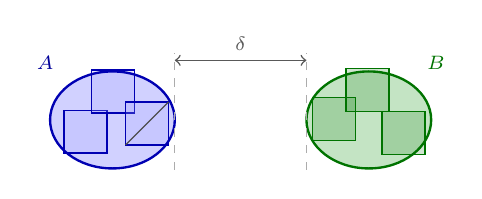
\begin{tikzpicture}[
  scale=0.88,
  every node/.style={font=\scriptsize},
  setAfill/.style={fill=blue!65, fill opacity=0.28, draw=none},
  setBfill/.style={fill=green!55!black, fill opacity=0.23, draw=none},
  setAline/.style={draw=blue!70!black, line width=0.85pt},
  setBline/.style={draw=green!45!black, line width=0.85pt},
  cellA/.style={fill=blue!35, fill opacity=0.22, draw=blue!70!black, line width=0.5pt},
  cellB/.style={fill=green!45!black, fill opacity=0.18, draw=green!45!black, line width=0.5pt},
  guide/.style={draw=gray!65, dashed, line width=0.45pt},
  measure/.style={<->, gray!70!black, line width=0.55pt},
  diamline/.style={gray!60!black, line width=0.45pt}
]
  \path[setAfill] (-1.85,0) ellipse [x radius=0.90, y radius=0.70];
  \path[setBfill] (1.85,0) ellipse [x radius=0.90, y radius=0.70];

  \foreach \x/\y in {-2.55/-0.48,-2.15/0.10,-1.66/-0.36}{
    \draw[cellA] (\x,\y) rectangle ++(0.62,0.62);
  }

  \foreach \x/\y in {1.04/-0.30,1.52/0.12,2.04/-0.50}{
    \draw[cellB] (\x,\y) rectangle ++(0.62,0.62);
  }

  \draw[setAline] (-1.85,0) ellipse [x radius=0.90, y radius=0.70];
  \draw[setBline] (1.85,0) ellipse [x radius=0.90, y radius=0.70];

  \draw[guide] (-0.95,-0.72) -- (-0.95,0.96);
  \draw[guide] (0.95,-0.72) -- (0.95,0.96);
  \draw[measure] (-0.95,0.86) -- (0.95,0.86)
    node[midway, above] {$\delta$};

  \draw[diamline] (-1.66,-0.36) -- (-1.04,0.26);

  \node[blue!60!black] at (-2.82,0.82) {$A$};
  \node[green!45!black] at (2.82,0.82) {$B$};
\end{tikzpicture}

  \caption{Positive distance separates cells with $\diam I_k<\delta$.}
  \label{fig:positive-distance-cell-cover-split}
\end{figure}

\begin{theorem} \label{thm:outer-measure-positive-distance-additivity} \hlt{Additivity at Positive Distance}\\
Let $A,B\subseteq\R^p$ be nonempty and disjoint, and suppose $\operatorname{dist}(A,B)\defeq\inf\{\norm{a-b}_2:a\in A,\ b\in B\}>0$.\\
Then $m_p^\ast(A\cup B)=m_p^\ast(A)+m_p^\ast(B)$.
\begin{proof}
The inequality $\leq$ follows from Theorem \ref{thm:cell-cover-outer-measure-basic-properties}. For $\geq$, set $\delta\defeq\operatorname{dist}(A,B)$. If $m_p^\ast(A\cup B)=+\infty$, done.\\
Otherwise, given $\varepsilon>0$, choose $(I_n)\in\mathcal{C}(A\cup B)$ with $\operatorname{diam}I_n<\delta$ and $\sum_n\operatorname{vol}_p(I_n)\leq m_p^\ast(A\cup B)+\varepsilon$.\\
Put $N_A\defeq\{n:I_n\cap A\neq\emptyset\}$ and $N_B\defeq\{n:I_n\cap B\neq\emptyset\}$. Since $N_A\cap N_B=\emptyset$, $(I_n)_{n\in N_A}$ covers $A$, $(I_n)_{n\in N_B}$ covers $B$, and $m_p^\ast(A)+m_p^\ast(B)\leq\sum_{n\in N_A}\operatorname{vol}_p(I_n)+\sum_{n\in N_B}\operatorname{vol}_p(I_n)\leq\sum_n\operatorname{vol}_p(I_n)\leq m_p^\ast(A\cup B)+\varepsilon$. Let $\varepsilon\downarrow0$.\\
\hlt{Structural Commentary}: Positive separation lets a sufficiently fine cover be sorted unambiguously.\\
\hlt{Key Insight}: Countable subadditivity becomes equality when no small cell can touch both pieces.
\end{proof}
\end{theorem}

\begin{theorem} \label{thm:outer-measure-agrees-with-cell-volume} \hlt{Outer Measure of a Cell}\\
If $I$ is a cell in $\R^p$, then $m_p^\ast(I)=\operatorname{vol}_p(I)$.
\begin{proof}
The cover $(I,\emptyset,\ldots)$ gives $m_p^\ast(I)\leq\operatorname{vol}_p(I)$. For $\geq$, the case $\operatorname{vol}_p(I)=0$ follows by nonnegativity.\\
Assume $\operatorname{vol}_p(I)>0$ and fix $\varepsilon>0$. Choose a closed cell $J\subseteq I$ with $\operatorname{vol}_p(I)-\varepsilon<\operatorname{vol}_p(J)$, taking $J=I$ when $I$ is closed. For any open-cell cover $(G_k)$ of $I$, compactness gives $J\subseteq\bigcup_{k=1}^{m}G_k$.\\
Let $\mathcal{Q}$ be the finite rectangular grid determined by the faces of $J,\overline{G_1},\ldots,\overline{G_m}$. Up to zero-volume boundary atoms, each $Q\in\mathcal{Q}$ with $Q\subseteq J$ lies in some $G_k$, hence $\operatorname{vol}_p(J)\leq\sum_{k=1}^{m}\operatorname{vol}_p(G_k)\leq\sum_{k=1}^{\infty}\operatorname{vol}_p(G_k)$.\\
Infimize over open-cell covers, use Proposition \ref{prop:outer-measure-cover-normalizations}, and let $\varepsilon\downarrow0$.\\
\hlt{Structural Commentary}: Compact inner cells reduce covers to finite grids.\\
\hlt{Key Insight}: Outer measure is calibrated so that cells keep their original volume.
\end{proof}
\end{theorem}

\begin{theorem} \label{thm:outer-measure-translation-invariance} \hlt{Translation Invariance of Outer Measure}\\
For $E\subseteq\R^p$ and $t\in\R^p$, $m_p^\ast(t+E)=m_p^\ast(E)$.
\begin{proof} The map $\mathcal{C}(E)\to\mathcal{C}(t+E)$, $(I_k)\mapsto(t+I_k)$, is bijective with inverse $(J_k)\mapsto(-t+J_k)$.\\
By Proposition \ref{prop:cell-volume-translation-invariant}, $\sum_k\operatorname{vol}_p(t+I_k)=\sum_k\operatorname{vol}_p(I_k)$, so the two infima are equal.\\
\hlt{Structural Commentary}: Translate covers forward and backward.\\
\hlt{Key Insight}: Translation invariance of cell volume lifts directly to translation invariance of outer measure.
\end{proof}
\end{theorem}

\begin{definition} \label{def:outer-measure-and-rudin-measurable-sets} \hlt{Outer Measure and $\mu$-Measurable Sets}\\
Let $\mu$ be additive, regular, nonnegative, and finite on $\mathcal{E}$.\\
For $E\subseteq\R^p$, define $\mu^\ast(E)\defeq\inf\sum\limits_{n=1}^{\infty}\mu(A_n)$, where infimum is over open elementary covers $E\subseteq\bigcup\limits_{n=1}^{\infty}A_n$.\\
For $A,B\subseteq\R^p$, set $A\triangle B\defeq(A\setminus B)\cup(B\setminus A)$ and $d_\mu(A,B)\defeq\mu^\ast(A\triangle B)$.\\
A set is \hlt{finitely $\mu$-measurable} if it is a $d_\mu$-limit of elementary sets.\\
It is \hlt{$\mu$-measurable} if it is a countable union of such sets; denote the classes by $\mathcal{M}_F(\mu)$ and $\mathcal{M}(\mu)$.
\end{definition}

\begin{definition} \label{def:tao-box-cover-outer-measure} \hlt{Box-Cover Outer Measure Model}\\
An \hlt{open box} in $\R^n$ is $B=\prod\limits_{i=1}^{n}(a_i,b_i)=\{(x_1,\ldots,x_n)\in\R^n:x_i\in(a_i,b_i) \ \forall i \}$, $b_i\geq a_i$, $\operatorname{vol}_n(B)\defeq\prod\limits_{i=1}^{n}(b_i-a_i)$.\\
For $\Omega\subseteq\R^n$, the \hlt{box-cover outer measure} is $m_n^\ast(\Omega)\defeq\inf\left\{\sum_{j\in J}\operatorname{vol}_n(B_j):(B_j)_{j\in J}\text{ covers }\Omega,\ J\text{ at most countable}\right\}$.
\end{definition}

\begin{figure}[H]
  \centering
  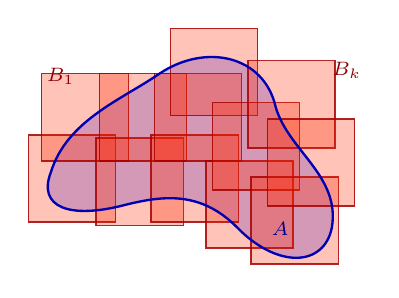
\begin{tikzpicture}[
  scale=0.82,
  every node/.style={font=\scriptsize},
  cover/.style={fill=red!70!orange, fill opacity=0.28, draw=red!65!black, draw opacity=0.85, line width=0.55pt},
  setfill/.style={fill=blue!65, fill opacity=0.34, draw=none},
  setoutline/.style={draw=blue!70!black, line width=0.85pt}
]
  \def\Ashape{%
    (-2.30,-0.42)
      .. controls (-2.05,0.38) and (-1.20,0.70) .. (-0.62,1.10)
      .. controls (0.10,1.58) and (1.00,1.38) .. (1.18,0.58)
      .. controls (1.38,-0.10) and (2.18,-0.48) .. (2.05,-1.28)
      .. controls (1.93,-1.90) and (1.20,-1.92) .. (0.58,-1.28)
      .. controls (0.02,-0.72) and (-0.55,-0.78) .. (-1.18,-0.94)
      .. controls (-2.00,-1.15) and (-2.52,-0.98) .. (-2.30,-0.42)
      -- cycle%
  }

  \path[setfill] \Ashape;

  \foreach \x/\y in {
    -2.65/-1.20,
    -2.45/-0.25,
    -1.60/-1.25,
    -1.55/-0.25,
    -0.75/-1.20,
    -0.70/-0.25,
    -0.45/0.45,
    0.10/-1.60,
    0.20/-0.70,
    0.75/-0.05,
    0.80/-1.85,
    1.05/-0.95
  }{
    \draw[cover] (\x,\y) rectangle ++(1.35,1.35);
  }

  \draw[setoutline] \Ashape;

  \node[blue!55!black] at (1.25,-1.30) {$A$};
  \node[red!55!black] at (-2.15,1.06) {$B_1$};
  \node[red!55!black] at (2.28,1.15) {$B_k$};
\end{tikzpicture}

  \caption{Cover $A\subseteq\bigcup_k B_k$ by squares; minimize $\sum_k\abs{B_k}$.}
  \label{fig:outer-measure-rectangle-cover}
\end{figure}

\begin{perspective} \label{per:outer-measure-geometric-box-covers} \hlt{Outer Measure as Outside Approximation}\\
Outer measure covers $A$ from outside; $d_\mu(A,B)=\mu^\ast(A\triangle B)$ measures closeness.\\
\hlt{Key Insight}: Countable subadditivity collects near-optimal covers.
\end{perspective}

\begin{method} \label{meth:lebesgue-measure-construction} \hlt{Lebesgue Measure Construction}
\begin{enumerate}[label=(\roman*)]
\setlength{\itemsep}{0pt}
\item \hlt{Cover from outside}\\
For $A\subseteq\R^n$, define $m_n^\ast(A)\defeq\inf\left\{\sum_{j\in J}\operatorname{vol}_n(B_j):(B_j)_{j\in J}\text{ covers }A,\ J\text{ at most countable}\right\}$.\\
This is defined for every set, but it is only countably subadditive in general.
\item \hlt{Keep the clean splitters}\\
Call $A$ measurable when every test set $X\subseteq\R^n$ splits additively: $m_n^\ast(X)=m_n^\ast(X\cap A)+m_n^\ast(X\cap A^c)$.\\
These measurable sets form a $\sigma$-algebra.
\item \hlt{Restrict the outer measure}\\
Define Lebesgue measure on measurable sets by $m(A)\defeq m_n^\ast(A)$.\\
On this restricted class, $m$ is countably additive.
\end{enumerate}
\hlt{Key Insight}: Outer measure sizes all sets; clean splitting restores additivity.
\end{method}

\begin{theorem} \label{thm:measure-measurability-main-source-todo}\label{thm:rudin-measure-extension} \hlt{Extension to a Measure}\\
Let $\mu$ be additive, regular, nonnegative, and finite on $\mathcal{E}$. Form $\mu^\ast$ from open elementary covers, set $d_\mu(A,B)=\mu^\ast(A\triangle B)$, and let $\mathcal{M}(\mu)$ be the countable unions of $d_\mu$-limits of elementary sets. Then:
\begin{enumerate}[label=(\roman*)]
\setlength{\itemsep}{0pt}
\item $\mu^\ast(A)=\mu(A)$ for $A\in\mathcal{E}$;
\item $\mu^\ast$ is countably subadditive;
\item $\mathcal{M}(\mu)$ is a $\sigma$-ring;
\item $\mu^\ast$ is countably additive on $\mathcal{M}(\mu)$.
\end{enumerate}
\begin{proof}
\begin{enumerate}[label=(\roman*)]
\setlength{\itemsep}{0pt}
\item Regularity gives $\mu^\ast(A)\leq\mu(A)$; compact closed approximants inside $A$ give the reverse inequality.
\item Cover each $E_n$ within $2^{-n}\varepsilon$ of $\mu^\ast(E_n)$; the combined cover proves subadditivity.
\item If $A_k\to A$, $B_k\to B$ in $d_\mu$, $A_k,B_k\in\mathcal{E}$, then $d_\mu(A_k\diamond B_k,A\diamond B)\leq d_\mu(A_k,A)+d_\mu(B_k,B)\to0$, $\diamond\in\{\cup,\cap,\setminus\}$.\\
Thus $\mathcal{M}_F(\mu)$ is a ring. If $A=\bigcup_kA_k$ with $A_k\in\mathcal{M}_F(\mu)$, then $A\setminus B=\bigcup_k(A_k\setminus B)$, so $\mathcal{M}(\mu)$ is a $\sigma$-ring.
\item For $A=\bigsqcup\limits_n A_n$, $A_n\in\mathcal{M}_F(\mu)$, subadditivity gives $\leq$,\\
while finite additivity gives $\mu^\ast(A)\geq\mu^\ast\left(\bigsqcup\limits_{n=1}^{N}A_n\right)=\sum\limits_{n=1}^{N}\mu^\ast(A_n)$.\\
Let $N\to\infty$, then decompose general disjoint families in $\mathcal{M}(\mu)$ into finite-measurable pieces.
\end{enumerate}
\hlt{Structural Commentary}: Elementary sets are completed under the distance measured by symmetric difference.\\
\hlt{Key Insight}: Approximate by elementary sets, prove identities there, then pass through $d_\mu(A,B)$.
\end{proof}
\end{theorem}

\begin{definition} \label{def:extended-and-lebesgue-measure} \hlt{Extended and Lebesgue Measure}\\
The \hlt{extended measure} is $\mu^\ast|_{\mathcal{M}(\mu)}$, denoted again by $\mu$.\\
For the elementary volume $m$, it is \hlt{Lebesgue measure} on $\R^p$.
\end{definition}

\begin{definition} \label{def:abstract-outer-measure-clean-division} \hlt{Abstract Outer Measure and Clean Division}\\
An \hlt{abstract outer measure} on $M$ is a monotone, countably subadditive function $\omega:2^M\to[0,+\infty]$ with $\omega(\emptyset)=0$.\\
A set $E\subseteq M$ is \hlt{$\omega$-measurable} if it cleanly splits every $X\subseteq M$: $\omega(X)=\omega(X\cap E)+\omega(X\cap E^c)$.\\
For Lebesgue outer measure, this is Caratheodory measurability.
\end{definition}

\begin{lemma} \label{lem:caratheodory-finite-measure-test} \hlt{Finite-Measure Test for Caratheodory Measurability}\\
Let $\omega:2^M\to[0,+\infty]$ be an outer measure. Then $E\subseteq M$ is $\omega$-measurable iff, for all $X\subseteq M$,\\
$\omega(X)<+\infty\Longrightarrow \omega(X)\geq\omega(X\cap E)+\omega(X\cap E^c)$.
\begin{proof}
\begin{enumerate}[label=\roman*.]
\setlength{\itemsep}{0pt}
\item[$(\Rightarrow)$] If $E$ is $\omega$-measurable, then $\omega(X)=\omega(X\cap E)+\omega(X\cap E^c)$ $\forall X\subseteq M$, hence finite-test inequality holds.
\item[$(\Leftarrow)$] For all $X\subseteq M$, $X=(X\cap E)\sqcup(X\cap E^c)$ gives $\omega(X)\leq\omega(X\cap E)+\omega(X\cap E^c)$. If $\omega(X)<+\infty$, the hypothesis gives $\geq$; if $\omega(X)=+\infty$, $\geq$ is automatic in $[0,+\infty]$. Thus equality holds for every $X$.
\end{enumerate}
\hlt{Structural Commentary}: To verify a clean split, only finite outer-measure test sets need real work.\\
\hlt{Key Insight}: Subadditivity supplies one inequality for free.
\end{proof}
\end{lemma}

\begin{figure}[H]
  \centering
  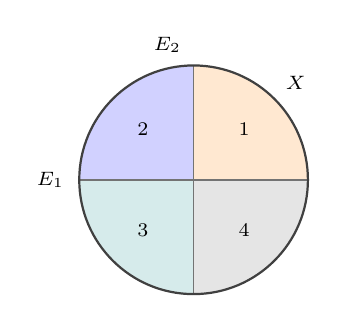
\begin{tikzpicture}[
  scale=0.88,
  every node/.style={font=\scriptsize},
  cut/.style={black!55, line width=0.65pt},
  boundary/.style={black!75, line width=0.8pt}
]
  \begin{scope}
    \clip (0,0) circle (1.65);
    \fill[orange!18] (0,0) rectangle (1.65,1.65);
    \fill[blue!18] (-1.65,0) rectangle (0,1.65);
    \fill[teal!16] (-1.65,-1.65) rectangle (0,0);
    \fill[black!10] (0,-1.65) rectangle (1.65,0);
    \draw[cut] (-1.65,0) -- (1.65,0);
    \draw[cut] (0,-1.65) -- (0,1.65);
  \end{scope}

  \draw[boundary] (0,0) circle (1.65);

  \node at (0.73,0.73) {$1$};
  \node at (-0.73,0.73) {$2$};
  \node at (-0.73,-0.73) {$3$};
  \node at (0.73,-0.73) {$4$};

  \node[above left=1pt] at (0,1.65) {$E_2$};
  \node[left=2pt] at (-1.65,0) {$E_1$};
  \node[above right=1pt] at (1.15,1.12) {$X$};
\end{tikzpicture}

  \caption{Two cuts split $X$ into four regions; $E_1\setminus E_2$ is region $2$.}
  \label{fig:measurable-difference-four-regions}
\end{figure}

\begin{definition} \label{def:outer-measure-zero-sets} \hlt{Zero Sets}\\
For outer measure $\omega:2^M\to[0,+\infty]$, \hlt{$\omega$-zero set} is $Z\subseteq M$ with $\omega(Z)=0$; $\mathcal{Z}_\omega\defeq\{Z\subseteq M:\omega(Z)=0\}$.
\end{definition}

\begin{theorem} \label{thm:caratheodory-measurable-sets-sigma-algebra} \hlt{Caratheodory Measurable Sets}\\
Let $\omega:2^M\to[0,+\infty]$ be an outer measure, and let $\mathcal{M}_\omega$ be the class of $\omega$-measurable subsets of $M$.\\
Then $\mathcal{M}_\omega$ is a $\sigma$-algebra, $\omega|_{\mathcal{M}_\omega}$ is countably additive, $\mathcal{Z}_\omega\subseteq\mathcal{M}_\omega$, and $E\in\mathcal{M}_\omega$, $Z\in\mathcal{Z}_\omega$\\
imply $E\cup Z,E\setminus Z,E\triangle Z\in\mathcal{M}_\omega$ and $\omega(E\cup Z)=\omega(E\setminus Z)=\omega(E\triangle Z)=\omega(E)$.
\begin{proof}
If $Z\in\mathcal{Z}_\omega$, then $\omega(X)\leq\omega(X\cap Z)+\omega(X\cap Z^c)\leq0+\omega(X)$, so $Z\in\mathcal{M}_\omega$. Complements are immediate.\\
If $E,F\in\mathcal{M}_\omega$, iterating the two clean cuts gives $\omega(X)=\sum_{\epsilon,\eta\in\{0,1\}}\omega(X\cap E^\epsilon\cap F^\eta)$, where $E^1=E$, $E^0=E^c$; hence all finite Boolean combinations of $E,F$ are measurable.\\
For disjoint $E_i\in\mathcal{M}_\omega$, set $E=\bigsqcup_iE_i$ and $F_N=(\bigcup_{i=1}^{N}E_i)^c$.\\
Finite splitting gives $\omega(X)=\sum_{i=1}^{N}\omega(X\cap E_i)+\omega(X\cap F_N)\geq\sum_{i=1}^{N}\omega(X\cap E_i)+\omega(X\cap E^c)$.\\
Letting $N\to\infty$ and using subadditivity for the reverse inequality yields $\omega(X)=\sum_{i=1}^{\infty}\omega(X\cap E_i)+\omega(X\cap E^c)$; hence $E\in\mathcal{M}_\omega$, and $X=E$ gives countable additivity.\\
General countable unions follow from $F_1=E_1$, $F_n=E_n\setminus\bigcup_{i<n}E_i$.\\
Finally, if $E\in\mathcal{M}_\omega$ and $Z\in\mathcal{Z}_\omega$, then $E=(E\setminus Z)\sqcup(E\cap Z)$ and $E\cup Z=E\sqcup(Z\setminus E)$ give $\omega(E\setminus Z)=\omega(E)$ and $\omega(E\cup Z)=\omega(E)$; also $E\triangle Z=(E\setminus Z)\sqcup(Z\setminus E)$ has measure $\omega(E)$.\\
\hlt{Structural Commentary}: Measurable sets preserve countable additivity.\\
\hlt{Key Insight}: Measurable cuts turn subadditivity into equality.
\end{proof}
\end{theorem}

\begin{definition} \label{def:lebesgue-sigma-algebra-caratheodory} \hlt{Lebesgue $\sigma$-Algebra via Caratheodory}
\begin{enumerate}[label=(\roman*)]
\setlength{\itemsep}{0pt}
\item $\mathcal{L}^n\defeq\{E\subseteq\R^n:E$ is $m_n^\ast$-measurable$\}$ is the \hlt{Lebesgue $\sigma$-algebra}.
\item $m\defeq m_n^\ast|_{\mathcal{L}^n}$ is \hlt{Lebesgue measure}; for $E\in\mathcal{L}^n$, write $m(E)=m_n^\ast(E)$.
\end{enumerate}
\end{definition}

\begin{proposition} \label{prop:cells-lebesgue-measurable-volume} \hlt{Cells Are Lebesgue Measurable}\\
For every coordinate cell $I\subseteq\R^n$, $I\in\mathcal{L}^n$ and $m(I)=\operatorname{vol}_n(I)$.
\begin{proof}
Since $I\in\mathcal{E}$, Theorem \ref{thm:rudin-measure-extension} gives $I\in\mathcal{L}^n$ and $m(I)=m_n^\ast(I)=\operatorname{vol}_n(I)$.\\
For the open-cell split, fix $A\subseteq\R^n$ with $m_n^\ast(A)<+\infty$.\\
Set $I_k\defeq\{x\in I:\operatorname{dist}(x,I^c)>k^{-1}\}$, $\eta_k\defeq m_n^\ast(I\setminus I_k)\to0$. Since $\operatorname{dist}(A\cap I_k,A\setminus I)>0$, Theorem \ref{thm:outer-measure-positive-distance-additivity} gives $m_n^\ast(A)\geq m_n^\ast(A\cap I_k)+m_n^\ast(A\setminus I)\geq m_n^\ast(A\cap I)+m_n^\ast(A\setminus I)-\eta_k$; let $k\to\infty$ and apply Lemma \ref{lem:caratheodory-finite-measure-test}.\\
\hlt{Structural Commentary}: Cells are the bridge between coordinate volume and Lebesgue measure.\\
\hlt{Key Insight}: Shrink, split, let the collar vanish.
\end{proof}
\end{proposition}
